\chapter{Plūsmas analīzes algoritma implementācija}
Plūsmas analīzes algoritma implementācija tika veidota programmēšanas valodā \textit{Python}, izmantojot \textit{caffe}. Šis ietvars tika izmantots, lai veiktu \textit{VGG Net} konvolūcijas neironu tīkla modelēšanu un apmācību objektu klasificēšanai un implementētu \textit{SSD} algoritmu objektu detektēšanai. Lai gan gala risinājums tika veidots izmantojot \textit{SSD} algoritmu, lai rastu plašāku ieskatu pieejamajos risinājumus, tika apskatīts arī \textit{YOLO} objektu detektēšanas algoritms, kas implementēts \textit{darknet} ietvarā.

Neatkarīgi no objektu detektēšanas algoritma un ietvara, kurā tas implementēts, gala risinājums sastāv no četrām daļām: datu kopas sagatavošanas, konvolūcijas neironu tīkla apmācības, objektu detektēšanas algoritma implementācijas un sekošanas algoritma implementācijas. Pēc datu sagatavošanas, tiek veikta konvolūcijas neironu tīkla apmācība,  lai tas būtu spējīgs klasificēt attēlos vai video fragmentos esošos objektus. Kad apmācīts pietiekami precīzs modelis, to katrā kadrā izmanto objektu detektēšanas algoritms, lai meklētu objektus. Kad objekts atrasts, tā vietā tiek inicializēts sekošanas algoritms, kas nākamajos kadros noteiks objekta atrašanās vietu, ja to vairs nebūs iespējams detektēt. 
\section{Cilvēku galvas noteikšanas datu sagatavošana}
Lai veiksmīgi apmācītu konvolūcijas neironu tīklus objektu detektēšanai, ir nepieciešama liela datu kopa ar meklējamo objektu piemēriem, šajā gadījumā ar cilvēku galvu attēliem. Jo vairāk datu, jo dažādākus objektus apmācītais tīkls spēs klasificēt. Šī darba nolūkos interesējošie piemēri ir cilvēku galvu attēli un ir pieejamas vairākas datu kopas, autors šī darba nolūkos ir izvēlējies \textit{HollywoodHeads} datu kopu \cite{vu15heads}. 

\textit{HollywoodHeads} datu kopa satur 369 846 cilvēku galvu anotācijas (anotācija ir \textit{XML} formāta fails, kas piekārtots katram datu kopas attēlam un satur informāciju par attēlu, par objektu, kādi objekti redzami attēlā un šo objektu ierobežojošie logi), 224 740 video kadros no 21 Holivudas filmām\footnote{Filmu saraksts: American beauty, As Good As It Gets, Big Fish, Big Lebowski, Bringing out the
dead, Capote, Clerks, Crash, Dead Poets Society, Double Indemnity, Erin
Brockovich, Fantastic 4, Fargo, Fear And Loathing In Las Vegas, Fight	Club,Five Easy Pieces, Forrest Gump, Gang Related, Gandhi, Charade, I Am Sam}. Šīs filmas ir no dažādiem žanriem un laika brīžiem vēsturē, lai piedāvātu visdažādākos galvu piemērus. Lai izveidotu anotācijas, datu kopas veidotāji manuāli atlasīja cilvēku galvas no rīcības bagātām ainām. Katrai galvai manuāli tika izveidoti ierobežojošie logi (mazākais iespējamais laukums, kurā ietilpst visi galvas redzamie pikseļi), vairāku kadru garumā. Kopā tika savākti dati no 2 380 klipiem ar 3 872 apsekotiem cilvēkiem, kas kopā veido vairāk kā 3.5 stundas ar video fragmentiem. Datu kopa ir sadalīta apmācības, validācijas un testēšanas apakškopās un šīs apakškopas, filmu ziņā, nepārklājas. \textit{HollywoodHeads} apmācības datu apakškopa satur 216 719 kadrus no 15 filmām, validācijas apakškopa satur 6 719 kadrus no 3 filmām un testēšanas apakškopa satur 1 302 kadrus no 3 filmām. Cilvēku galvas, kurām priekšā ir šķēršļi vai ir slikts apgaismojums ir anotācijās apzīmētas kā "sarežģīti" (no angļu val. \textit{difficult}) piemēri un netiek izmantoti apmācības laikā. 

Diemžēl, izvēlēto datu kopu gan nav iespējams uzreiz pielietot apmācībā, jo formāts kādā strukturēti dati vienmēr nav saderīgs ar formātu kādu sagaida ietvars, šajā gadījumā \textit{caffe} un \textit{darknet}. Konvolūciju neironu tīklu apmācībā populāras datu kopas ir: \textit{COCO} \cite{lin2014microsoft}, \textit{PASCAL VOC} \cite{everingham2010pascal} un \textit{ILSVRC} \cite{ILSVRC15}. \textit{Caffe} un \textit{darknet} ietvaros ir iebūvēta iespēja apmācīt CNN ar visām minētajām datu kopām, izņemot \textit{HollywoodHeads} datu kopu. Šīs problēmas risinājums gan nav sarežģīts. Autors aizstāja \textit{VOC} datu kopas attēlus un anotācijas (anotāciju struktūra abām datu kopām sakrīt un specifiski anotāciju pārveidojumi nav nepieciešami) ar \textit{HollywoodHeads} datu kopas attēliem un anotācijām un gan \textit{caffe}, gan \textit{darknet} uzstādījumos bija nepieciešams nomainīt klašu skaitu. \textit{Caffe} gadījumā klašu skaits no 20 (\textit{VOC} gadījumā) tika samainīts uz 2 klasēm (galva un fons), kamēr \textit{darknet} gadījumā klašu skaits no 20 tika samainīts uz 1 klasi (galva).

Nākamais solis datu sagatavošanā \textit{caffe} ietvaram ir izveidot \textit{LMDB} (\textit{Lightning Memory-Mapped Database}), kurā iekodēs attēlu informāciju. \textit{LMDB} ir ļoti augstas veiktspējas, kompakta datu glabātuve, kas izmanto atmiņā kartētus failus, lai varētu lasīt datus ar augstu veiktspēju, tai pašā laikā saglabājot standarta uz diskiem balstīto datu glabātuvju ietilpību. Apmācības, validācijas un testēšanas datu apakškopām katrai būs sava \textit{LMDB} datu glabātuve ar saitēm uz pašu datu kopu. \textit{Bash} skripts, kas izveidos šīs datubāzes ir ievietots pielikumā \ref{appendix:pielikums1}. Papildus datubāzēm, lai sāktu apmācību ir nepieciešams ģenerēt teksta failus, kuros norādītas apmācības, validācijas un testēšanas attēlu atrašanās vietas datorā.

\textit{Darknet} ietvara gadījumā, no \textit{VOC} formāta datiem ir nepieciešams izveidot marķējumu (no angļu val. \textit{label}) failus, kas no anotāciju failiem iegūs attēlos esošo objektu ierobežojošo logu izmērus un atrašanās vietas un klasi kurām pieder šie logi. Marķējumu faili katrā rindā satur informāciju par vienu no ierobežojošajiem logiem, formātā :\\ $<objekta-klase> <x> <y> <platums> <augstums>$.\\
Kur \textit{x,y, platums, augstums} ir atkarīgi no attēla platuma un augstuma. Lai automātiski izveidotu marķējumu failus katram attēlam, ir nepieciešams palaist \textit{Python} programmēšanas valodā rakstītu skriptu, kas pievienots pielikumā \ref{appendix:pielikums2}. Šis skripts nolasa katru anotācijas failu un atkarībā no anotācijas failā atrastajiem parametriem, katram attēlam izveido marķējumu failu ar iepriekš minēto informāciju un izveido teksta failus, kuros norādītas apmācības, validācijas un testēšanas attēlu atrašanās vietas datorā. Kad šie datu glabātuvju un datu sadalījumu faili ir ģenerēti, ir iespējams sākt tīkla apmācību.
\section{Konvolūcijas neironu tīkla apmācība}
Lai veiksmīgi apmācītu konvolūciju neironu tīklus, ir nepieciešama ierīce ar jaudīgu \textit{GPU} jeb \textit{Graphics Processing Unit}. \textit{GPU} kalpo, lai skaitļošanas jaudu izdalītu datora jeb citu ierīču grafiskajiem procesoriem, kuri sastāv no simtiem kodolu un katrs kodols ir spējīgs paralēli izpildīt kādu darbību. Izmantojot \textit{CPU} jeb \textit{Central Processing Unit}, lietotājiem ir pieejami kodolu skaits sākot no 1 līdz 16. Šī darba nolūkos, konvolūciju neironu tīkli tika apmācīti izmantojot \textit{NVIDIA GeForce GTX 1080} grafisko procesoru, kam pieejami 2 560 kodoli un 8 GB operatīvā atmiņa. Apmācības procesa konfigurēšana katram ietvaram atšķiras.

\paragraph{\textit{SSD} detektēšanas sistēmas apmācība izmantojot \textit{caffe} ietvaru}
\hfill\par
Pēc datu sagatavošanas ir nepieciešams izvēlēties tīkla arhitektūru ar kuru notiks apmācība. \textit{Caffe} ietvarā ir ļoti elementāri izveidot pašam savu arhitektūru, taču nav iespējams paredzēt cik precīza būs šī arhitektūra, tāpēc labāk izvēlēties kādu no \textit{caffe} jau piedāvātajām, piemēram, \textit{GoogLeNet} vai \textit{AlexNet}. Ar darbā izmantoto grafisko skaitļošanas iekārtu nav iespējams efektīvi apmācīt ļoti sarežģītus tīklus, tāpēc \textit{SSD} apmācībā tika izmantota \textit{VGG Net} arhitektūra, ar kuru apmācības laiki nebūs ļoti gari un kas ir pielāgota \textit{caffe} ietvaram \cite{ssdmodel}. Pēdējās darbības pirms sākt apmācību ir risinātāja (no angļu val. \textit{solver}) un tīkla modeļa konfigurācijas failu pielabošana (ieskaitot apmācības parametrus kā filtru skaitu, klašu skaitu, cik attēlus vienlaicīgi piedāvāt apmācībai), lai apmācībai izmantotu pirms tam sagatavotos datus ar tikai vienu klasi. Pēdējais solis pirms apmācības sākšanas ir sākuma svaru iegūšana, kas ir publiski pieejami lejupielādei. Pēc sākuma svaru lejupielādēšanas, apmācība var sākties. 

\textit{SSD} gadījumā, lai zinātu, kad pārtraukt apmācību, autors novēroja \textit{mAP} jeb \textit{Mean Average Precision} metriku un \textit{loss} funkcijas atgrieztās vērtības, kad tās sāka tuvoties nullei, regulāri tika pārbaudīti attēli, kuros novērojamas galvas. Kad modelim piedāvātie attēli atgrieza apmierinošas vērtības, autors pieņēma, ka modelis ir pietiekami labi apmācīts, lai to izmantotu gala risinājumā. 
\begin{figure}[!htb]
	\minipage{0.50\textwidth}
	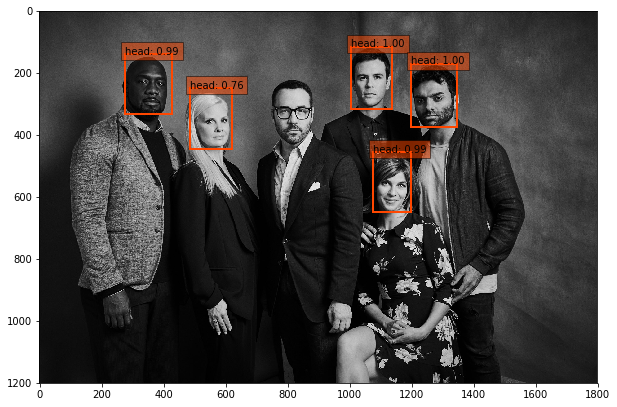
\includegraphics[width=\linewidth]{images/caffessd1.png}
	\caption{Melnbalts attēls, ko izmantoja modeļa pārbaudīšanai ar \textit{SSD} detektēto objektu ierobežojošajiem logiem}
	\endminipage\hfill
	\minipage{0.50\textwidth}%
	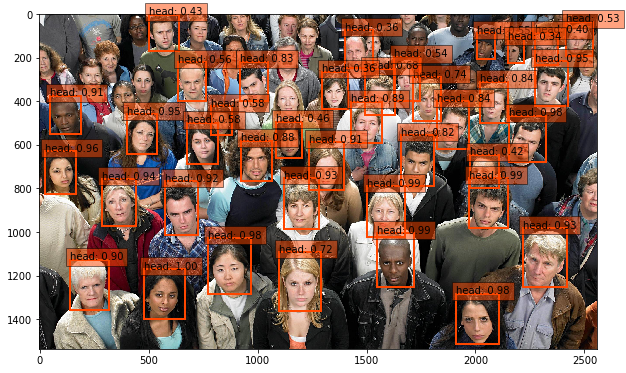
\includegraphics[width=\linewidth]{images/caffessd2.png}
	\caption{Augsta cilvēku blīvuma attēls, ko izmantoja modeļa pārbaudīšanai ar \textit{SSD} detektēto objektu ierobežojošajiem logiem}
	\endminipage
\end{figure}

Gan attēlā 3.1, gan attēlā 3.2 redzamie ierobežojošie logi norāda uz detektēšanas sistēmas atrastajiem objektiem. Minētajos attēlos var novērot, ka detektēšanas sistēma nav atradusi visus iespējamos objektus, bet ir atrasta vismaz lielākā daļa objektu un var pieņemt, ka tīkls ir pietiekami apmācīts, lai to izmantotu gala risinājumā. Kā iemeslus visu objektu neatrašanai var minēt melnbalto krāsu paleti attēlā 3.1 un augsto cilvēku izvietojuma blīvumu attēlā 3.2. 

\paragraph{\textit{YOLO} detektēšanas sistēmas apmācība izmantojot \textit{darknet} ietvaru}
\hfill\par
Pēc datu sagatavošanas, \textit{YOLO} konfigurācijas failos ir jānorāda kura tīkla arhitektūra tiks izmantota (\textit{darknet} piedāvā lielu apjomu ar \textit{YOLO} tīkla arhitektūru variācijām), kurā direktorijā atrodas apmācību dati, klašu skaits un jānorāda direktorija kur atrodas fails ar visu klašu nosaukumiem. Tika izveidoti 3 konfigurācijas faili: 
\begin{enumerate}
	\item norādes uz apmācības datu direktorijām un klašu skaitu; 
	\item visu klašu nosaukumiem;
	\item tīkla arhitektūra, kurā norādīti katra slāņa parametri;
\end{enumerate}

Pirmais minētais fails satur informāciju par klašu skaitu, norādi uz apmācības un validācijas failu apakškopām, norāde uz failu ar visu klašu nosaukumiem un norādi kur glabāt apmācītos modeļus. Šī darba nolūkos šis fails ir ar sekojošu struktūru: 
\begin{lstlisting} 
	classes= 1  
	train  = obj/2012_train.txt  
	valid  = obj/2012_test.txt  
	names = cfg/obj.names  
	backup = backup/
\end{lstlisting}

Fails ar visu klašu nosaukumiem ir ļoti vienkāršs, katrā jaunā rindā ir ierakstīts apmācības datos esošo klašu nosaukumi. Šī darba ietvaros šis fails satur tikai vienu ierakstu "head", kas apzīmē datu kopā esošos galvu attēlu piemērus.

Pēdējais minētais fails, ko nepieciešams sagatavot, lai sāktu apmācību ir tīkla arhitektūras konfigurācijas fails. Lai lieki nesarežģītu apmācības procesu, autors izmantoja \textit{darknet} ietvarā piedāvāto noklusējuma konfigurāciju un veica sekojošas izmaiņas:

\begin{enumerate}
	\item \textit{batch} mainīgais konfigurācijā tika nomainīts uz 64, kas apzīmē cik liela attēlu kopa tiks izmantota katrā apmācības solī. Jo lielāku iestata šo vērtību, jo vairāk skaitļošanas resursus prasīs tīkla apmācība.
	\item \textit{subdivision} mainīgais konfigurācijā tika nomainīts uz 4, kas apzīmē, cik daļās tika sadalīta katra pirmajā punktā minētā attēlu kopa, lai izlīdzinātu \textit{GPU} operatīvās atmiņas patēriņu.
	\item \textit{classes} mainīgais konfigurācijā tika nomainīts uz 1, kas apzīmē cik klases tiks detektētas.
	\item \textit{filters} mainīgais pēdējā tīkla slānī tika nomainīts uz 30 pēc formulas $filters=(classes + 5)*5$
\end{enumerate}

Pēdējais solis pirms apmācības sākšanas ir sākuma svaru iegūšana, kas ir publiski pieejami lejupielādei. Pēc sākuma svaru lejupielādēšanas, apmācība var sākties. 

Līdzīgi kā \textit{SSD} gadījumā, arī apmācot \textit{YOLO} detektēšanas sistēmu, lai zinātu, kad pārtraukt apmācību, autors novēroja \textit{mAP} jeb \textit{Mean Average Precision} metriku un \textit{loss} funkcijas atgrieztās vērtības, kad tās sāka tuvoties nullei, regulāri tika pārbaudīti attēli, kuros novērojamas galvas. Kad modelim piedāvātie attēli atgrieza apmierinošas vērtības, autors pieņēma, ka modelis ir pietiekami labi apmācīts, lai to izmantotu gala risinājumā.

\begin{figure}[!htb]
	\minipage{0.50\textwidth}
	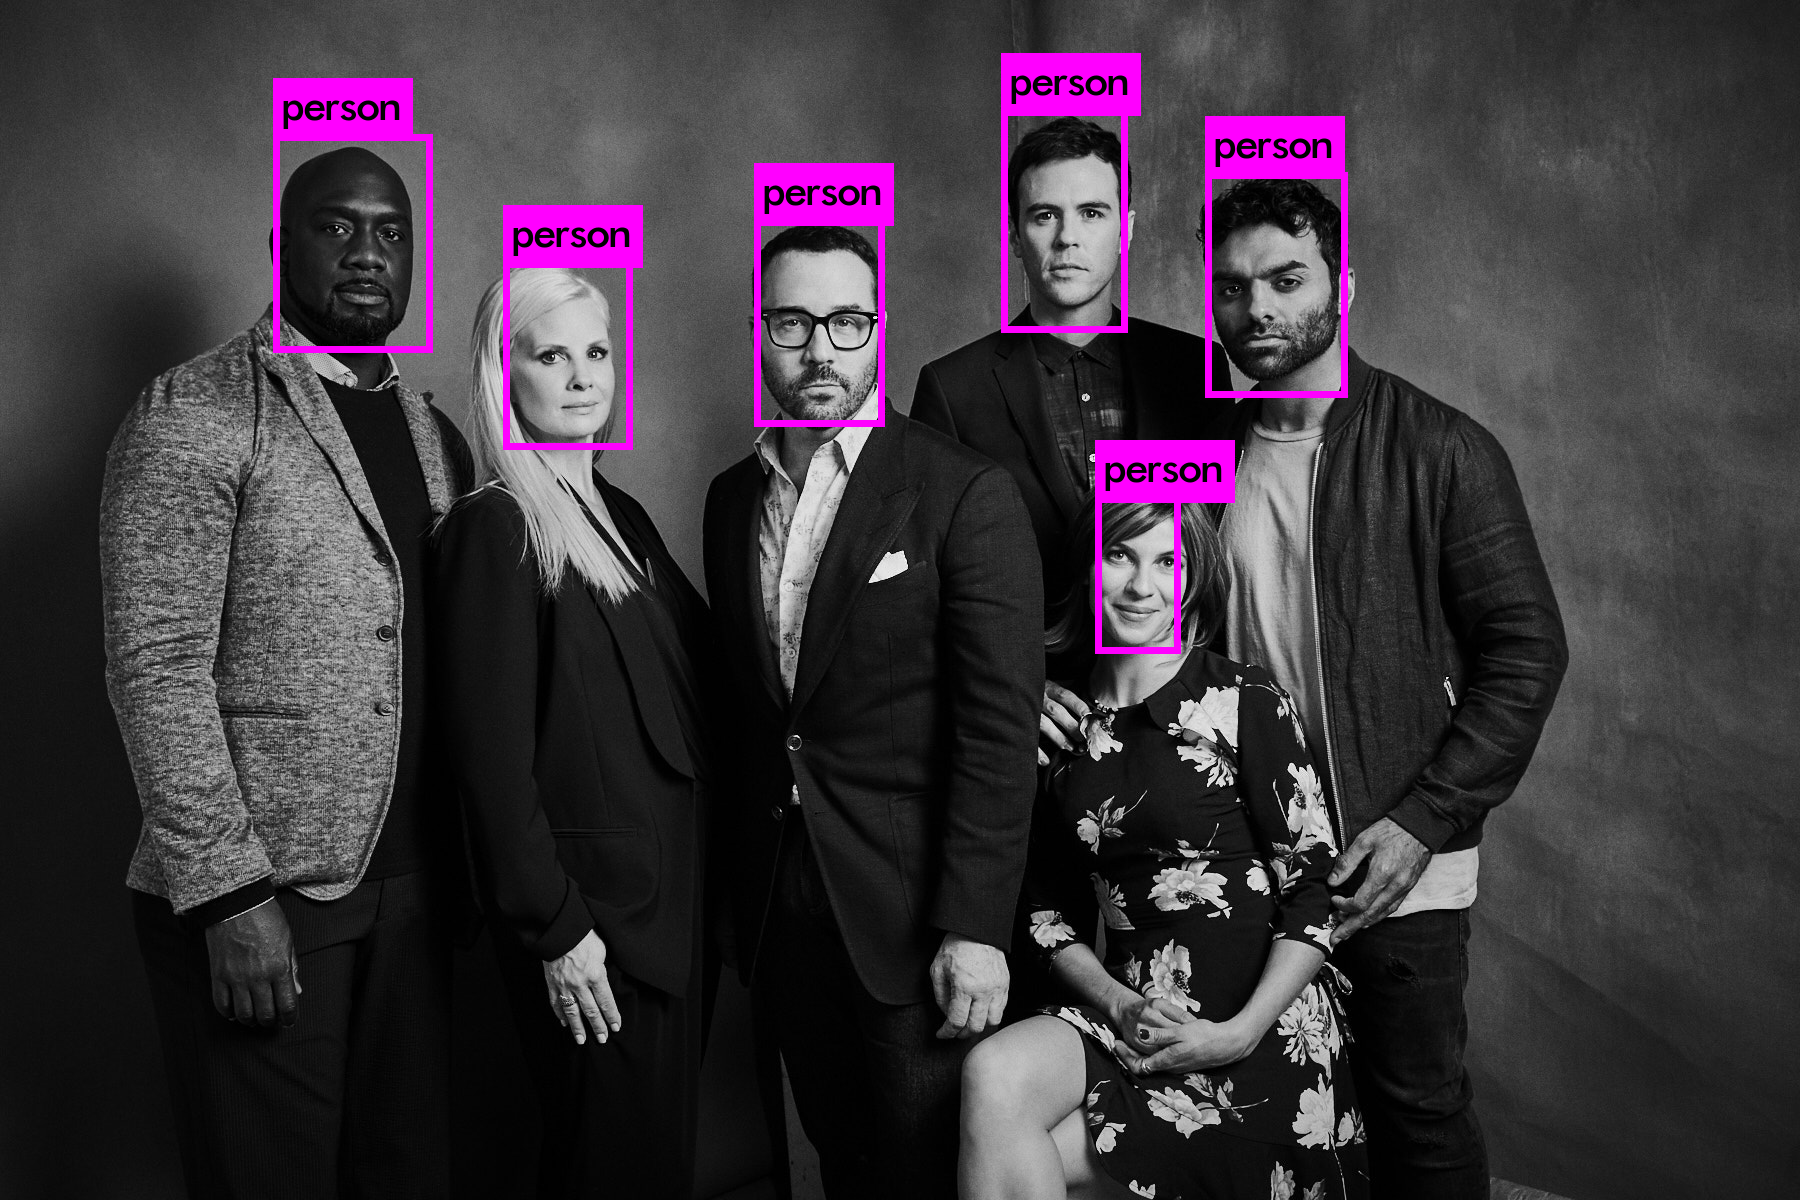
\includegraphics[width=\linewidth]{images/predictions.png}
	\caption{Melnbalts attēls, ko izmantoja modeļa pārbaudīšanai ar \textit{YOLO} detektēto objektu ierobežojošajiem logiem}
	\endminipage\hfill
	\minipage{0.50\textwidth}%
	\includegraphics[width=\linewidth]{images/predictions2.png}
	\caption{Augsta cilvēku blīvuma attēls, ko izmantoja modeļa pārbaudīšanai ar \textit{YOLO} detektēto objektu ierobežojošajiem logiem}
	\endminipage
\end{figure}

Attēlā 3.3, \textit{YOLO} objektu detektēšanas sistēma ir spējusi atrast visus 6 attēlā esošos, interesējošos objektus, kamēr attēlā ar augstu cilvēku blīvumu, detektēšana ir krietni vājāka. Kā iemeslu vājajai detektēšanai attēlos ar augstu cilvēku blīvumu, var minēt \textit{YOLO} algoritma nianses. Režģi, kuros sadala attēlu pārklājas vairākiem objektiem un \textit{YOLO} sagādā problēmas mazu objektu detektēšana. Šo problēmu var daļēji novērst, detektēšanas laikā, padot sistēmai attēlus ar augstāku izšķirtspēju, lai režģu izveidošana attēlam ir vienmērīgāka, taču šāds process tērētu lielākus skaitļošanas resursus. 
\section{Detektēšanas un sekošanas algoritmu implementācija}
Pēc tīkla apmācības gan \textit{caffe}, gan \textit{darknet} ietvars atgriež modeļus ar tīkla svariem. Izmantojot šos modeļus, ir iespējams veikt objektu detektēšanu attēlos. Abi ietvari piedāvā sagatavotas metodes objektu detektēšanai, balstoties uz no apmācības iegūtajiem modeļiem, programmēšanas valodā \textit{Python}. Šīs metodes abiem ietvariem ir pilnīgi atšķirīgas un tās apraksta abu detektēšanas algoritmu darbību. Ja neskaita labojumus, kas tika veikti sakarā ar detektēšanai padoto datu formātu un klašu skaitu, abu ietvaru piedāvātās metodes objektu detektēšanai darbojās un tām nebija nepieciešamas korekcijas. Gan \textit{caffe}, gan \textit{darknet} ietvari piedāvā \textit{detect} funkcijas, implementētas \textit{Python} programmēšanas valodā. Abiem ietvariem šīs funkcijas atgriež visu atrasto objektu ierobežojošo logu koordinātes, klases nosaukumu un ar kādu pārliecību sistēma domā, ka atrastais objekts pieder minētajai klasei. Vienīgā lieta kas mainās šo funkciju atgrieztajos rezultātos ir informācijas formatējums un gala risinājuma implementāciju tas ļoti neietekmē. Ņemot vērā minēto informāciju, var secināt, ka pēc detektēšanas posma, pārējā risinājuma implementācija abām detektēšanas sistēmām būs vienāda. Lai izvairītos no atkārtošanās, šīs sadaļas ietvaros tiks apskatīta tikai \textit{SSD} detektēšanas sistēmas un \textit{OpenCV} sekošanas algoritmu apvienošana vienā risinājumā, jo darba ietvaros \textit{SiamFC} algoritmu praktiski implementēt neizdevās, lai gan tika apskatīta šī algoritma implementācija \textit{PyTorch} un \textit{TensorFlow} ietvaros \cite{siamfcrepo1,siamfcrepo2}. 
\paragraph{Sekošana pēc detektēšanas ar \textit{OpenCV} bibliotēkā piedāvātajiem risinājumiem} 
\hfill\par
\textit{OpenCV} ir atvērtā koda datorredzes un mašīnmācīšanās programmatūras bibliotēka, kurā ir implementēti arī divi no trim darbā apskatītajiem sekošanas algoritmiem: \textit{MIL} jeb \textit{Multiple Instance Learning} un \textit{AdaBoost} sekošanas algoritmi. Pirmais solis sekošanas risinājuma izveidē ir video interesējošā reģiona izvēlēšanās (ir iespējams izvēlēties, ka detektēšana un sekošana nenotiek visā video laukumā, bet tikai daļā no video) un sekotāja (no angļu val. \textit{tracker}) uzstādīšana. Kad tas izdarīts, tiek atvērts video fragments un detektēšanas algoritms apskata vienu kadru pēc otra, līdz atrasts kāds no interesējošajiem objektiem, šajā gadījumā cilvēku galvas. Kad detektēšanas sistēma ir atradusi objektu, no objekta koordinātēm tiek izveidots ierobežojošais logs, tas tiek parādīts un notiek sekotāja inicializēšana šajā ierobežojošajā logā. Nākamajos kadros no jauna notiek objektu detektēšana un jaunu sekotāju inicializēšana un tiek atjaunotas iepriekšējos kadros izveidoto sekotāju atrašanās vietas.  

Papildus dažādu sekošanas algoritmu implementācijām, \textit{OpenCV} programmatūras bibliotēka piedāvā arī metodes, kas var atvieglot darbu ar attēliem un video fragmentiem kā arī kalpo datu vizualizācijai. Šīs metodes kā arī citas attēlu pārveidojumu operācijas netiks aprakstītas.

\begin{lstlisting} 
roi = cv2.selectROI(firstFrame,False)
line = cv2.selectROI(firstFrame,False)
tracker = cv2.MultiTracker_create()   
while(videoFile.isOpened()):  
	ret, frame = videoFile.read()     
	result = detection.detect(frame)    
\end{lstlisting}
Šajā koda fragmentā ir atlasītas svarīgas inicializācijas metodes. Šajās koda rindās uzskaitītas metodes, kas inicializē reģionu kurā veiks detektēšanu un sekošanu, kā arī līniju, kuru izmantos cilvēku skaitīšanai. Tiek inicializēts \textit{OpenCV} piedāvātais \textit{MultiTracker} objekts \cite{multitrack}, kas ļauj vienlaikus uzturēt vairākus aktīvus sekotājus. Ciklā tiek atvērts video fragments un atlasīts kadrs, kuram veic detektēšanas operāciju. Nākamās koda rindas darbojas ar detektēšanas procesā atrastajiem objektiem.

\begin{lstlisting}   
	if not boxCenters:
		tracker.add(cv2.TrackerMIL_create(), frame, bbox)
	else:
		newTracker = False
		distanceList = list()
		for cent in boxCenters:
			distanceList.append(math.sqrt( ((cent[0]-detectCenter[0])**2)+
											((cent[1]-detectCenter[1])**2)))
		if min(distanceList)>100:
			newTracker = True
	if newTracker:
		tracker.add(cv2.TrackerMIL_create(), frame, bbox)
ok, boxes = tracker.update(frame)
\end{lstlisting}

Šī koda daļa tiek izpildīta visiem detektēšanas laikā atrastajiem objektiem. Mainīgais \textit{boxCenters} satur sarakstu ar visu aktīvo sekotāju ierobežojošo logu viduspunktiem. Tiek pārbaudīts vai detektēšanas laikā atrastais objekts atrodas šajā sarakstā, ja nē, tad tiek noteikta atrastā objekta Eiklīda distance līdz visiem aktīvajiem sekotājiem un ja tā ir mazāka par 100, tad pieņem, ka detektētajam objektam līdz šim vēl netiek sekots un tiek inicializēts jauns sekotājs, ar 15. rindā redzamo komandu. Šajā brīdī izvēlas kādu no \textit{OpenCV} piedāvātajiem sekošanas algoritmiem izmantot. Šī darba ietvaros tiks salīdzināti \textit{OpenCV} piedāvātie \textit{TrackerMIL} (MIL sekošanas algoritms) un \textit{TrackerBoosting} (AdaBoost sekošanas algoritms) sekošanas algoritmu rezultāti. Pēdējā koda fragmenta rinda atjauno visus eksistējošos sekotājus ar jaunajām koordinātēm. 

Pēdējais posms gala risinājumā ir cilvēku skaitīšana. Līnijas izvēli izdara sistēmas lietotājs, diemžēl \textit{OpenCV} nepiedāvā funkcionalitāti izvēlēties interesējošo līniju, bet izmantojot \textit{OpenCV} piedāvāto reģiona izvēlēšanās funkcionalitāti \textit{selectROI} no atlasītā reģiona tiek savienoti \textit{(xmin,ymin)} ar \textit{(xmax,ymax)}, tādā veidā iegūstot līniju, kuru šķērsojot tiks skaitītas cilvēku galvas.
\newpage
\begin{lstlisting}
	boxCenters = list()
	for idx,newbox in enumerate(boxes):            
		p1 = (int(newbox[0]), int(newbox[1]))
		p2 = (int(newbox[0] + newbox[2]), int(newbox[1] + newbox[3]))
		center = ((int((newbox[0]+int(newbox[0] + newbox[2]))*0.5)),(int((newbox[1]+int(newbox[1] + newbox[3]))*0.5)))
		finishcenters.append(center)
		if (roi[1] < center[1] < roi[1]+roi[3] and roi[0] < center[0] < roi[0]+roi[2]) and ok:
		boxCenters.append(center)
		cv2.rectangle(frame, p1, p2, (0,255,0))
		if (countLine[0] is not None and idx<len(tempCenters) and idx<len(boxCenters)):
			if(tempCenters[idx][1]< countLine[0][1] and boxCenters[idx][1] >= countLine[0][1]) or 	(tempCenters[idx][1]<countLine[1][1] and boxCenters[idx][1] >= countLine[1][1]):
				count = count+1
\end{lstlisting}

Šis koda fragments uzzīmē vizualizācijā jaunās sekotāja ierobežojošos logus un pārbauda vai laikā starp iepriekšējo kadru un šī brīža kadru, sekotāju logu centri nav šķērsojoši iezīmēto līniju. Ja līnija ir šķērsota, tad tiek palielināts mainīgais, kas atbildīgs par skaitu. Pilnais \textit{SSD} detektēšanas sistēmas un sekošanas algoritmu implementācijas kods bez labojumiem ir pievienots pielikumā \ref{appendix:pielikums3} un \textit{YOLO} detektēšanas sistēmas implementācijas pilnais kods ir pievienots pielikumā \ref{appendix:pielikums4}.